% 压缩浮动体之间的间距
\setlength{\floatsep}{4pt plus 2pt minus 2pt}
\setlength{\textfloatsep}{6pt plus 2pt minus 2pt}
\setlength{\intextsep}{4pt plus 2pt minus 2pt}
\setlength{\abovecaptionskip}{3pt}
\setlength{\belowcaptionskip}{2pt}

\section{实验结果}

首先介绍我们的实验设置，对于SVM的训练方案，手势前后补充样本数量为100；对于基于CNN和频谱RGB图像的方案，采用MobileNet v2（在ImageNet 1K上预训练）进行全量微调，优化器使用Adam优化器；对于LSTM方法，采用input size=6, hidden\_size=60，同样采用Adam优化器，具体参数配置如下。

\begin{table}[h!]
    \centering
    \caption{\ptheadingfont{SVM训练配置}}
    \label{tab:svm_config}
    {\zihao{5}\setlength{\baselineskip}{1\baselineskip}%
    \begin{tabularx}{\linewidth}{|>{\centering\arraybackslash}p{3cm}|>{\centering\arraybackslash}p{2cm}|>{\centering\arraybackslash}X|>{\centering\arraybackslash}p{2cm}|}
        \hline
        \textbf{输入特征} & \textbf{填充Padding} & \textbf{分类器} & \textbf{Epoch} \\
        \hline
        41维（3$\times$13+2） & 100 & SVC(kernel=``rbf'', C=5)\newline + OneVsRestClassifier & 无epoch \\
        \hline
    \end{tabularx}}
\end{table}

\begin{table}[h!]
    \centering
    \caption{\ptheadingfont{CNN训练配置}}
    \label{tab:cnn_config}
    {\zihao{5}\setlength{\baselineskip}{1\baselineskip}%
    \begin{tabularx}{\linewidth}{|>{\centering\arraybackslash}p{1.6cm}|>{\centering\arraybackslash}X|>{\centering\arraybackslash}p{2.2cm}|>{\centering\arraybackslash}p{1.2cm}|>{\centering\arraybackslash}X|>{\centering\arraybackslash}p{2.2cm}|>{\centering\arraybackslash}p{1.2cm}|}
        \hline
        \textbf{输入维度} & \textbf{骨干网络} & \textbf{批次大小} & \textbf{优化器} & \textbf{优化器参数} & \textbf{学习率调度} & \textbf{Epoch} \\
        \hline
        $224\times224$ & \mbox{MobileNet\_V2}\newline\mbox{(ImageNet 1K)} & Train:8 /\newline Val:16 & Adam & \mbox{LR=3e-4,}\newline\mbox{WD=1e-4} & \mbox{step=10,}\newline\mbox{gamma=0.5} & 30 \\
        \hline
    \end{tabularx}}
\end{table}

\begin{table}[h!]
    \centering
    \caption{\ptheadingfont{LSTM训练配置}}
    \label{tab:lstm_config}
    {\zihao{5}\setlength{\baselineskip}{1\baselineskip}%
    \begin{tabularx}{\linewidth}{|>{\centering\arraybackslash}p{1.8cm}|>{\centering\arraybackslash}X|>{\centering\arraybackslash}p{1.6cm}|>{\centering\arraybackslash}p{1.2cm}|>{\centering\arraybackslash}X|>{\centering\arraybackslash}p{2.2cm}|>{\centering\arraybackslash}p{1.2cm}|}
        \hline
        \textbf{隐藏维度} & \textbf{网络结构} & \textbf{批次大小} & \textbf{优化器} & \textbf{优化器参数} & \textbf{损失函数} & \textbf{Epoch} \\
        \hline
        60 & \mbox{LSTM(6,60)}$\to$\newline\mbox{Linear(60,}\newline\mbox{num\_classes)} & 10 & Adam & \mbox{LR=3e-3,}\newline\mbox{WD=2e-3} & \mbox{CrossEntropy}\newline\mbox{Loss} & 30 \\
        \hline
    \end{tabularx}}
\end{table}

我们的测试结果如下所示，其中，SVM方法平均训练时间0.011s，CNN方法平均训练时间172.1s，LSTM平均训练时间为79.1s。

\begin{table}[h!]
    \centering
    \caption{\ptheadingfont{SVM vs. CNN vs. RNN/LSTM}}
    \label{tab:results}
    {\zihao{5}\setlength{\baselineskip}{1\baselineskip}\setlength{\tabcolsep}{3pt}%
    \begin{tabularx}{\linewidth}{|>{\centering\arraybackslash}p{0.8cm}|*{4}{>{\centering\arraybackslash}X}|*{4}{>{\centering\arraybackslash}X}|*{4}{>{\centering\arraybackslash}X}|}
        \hline
        & \multicolumn{4}{c|}{\textbf{SVM}} & \multicolumn{4}{c|}{\textbf{CNN}} & \multicolumn{4}{c|}{\textbf{LSTM}} \\
        \hline
        \textbf{Fold} & Acc & Prec & Rec & F1 & Acc & Prec & Rec & F1 & Acc & Prec & Rec & F1 \\
        \hline
        1 & 91.2 & 89.5 & 87.2 & 88.1 & 99.1 & 98.8 & 99.3 & 99.0 & 63.2 & 58.1 & 50.0 & 52.0 \\
        2 & 92.9 & 91.5 & 90.2 & 90.5 & 98.2 & 97.4 & 99.3 & 98.3 & 61.1 & 65.0 & 48.6 & 49.9 \\
        3 & 86.7 & 87.6 & 84.8 & 85.6 & 97.3 & 98.0 & 96.9 & 97.4 & 60.2 & 57.7 & 48.9 & 49.4 \\
        4 & 90.3 & 88.9 & 87.1 & 87.8 & 99.1 & 98.7 & 98.6 & 98.6 & 64.8 & 63.2 & 50.9 & 50.8 \\
        5 & 89.4 & 90.3 & 86.1 & 87.5 & 98.2 & 99.3 & 97.4 & 98.2 & 63.7 & 67.6 & 52.4 & 54.9 \\
        \hline
        \textbf{Avg.} & \textbf{90.1} & \textbf{89.6} & \textbf{87.1} & \textbf{87.9} & \textbf{98.4} & \textbf{98.5} & \textbf{98.3} & \textbf{98.3} & \textbf{62.5} & \textbf{62.3} & \textbf{50.2} & \textbf{51.4} \\
        \hline
    \end{tabularx}}
\end{table}

其中对于LSTM这种方法呈现的意外低准确率作出以下分析：1.数据量太小，而LSTM参数量较大，可能导致过拟合；2.时序长度不稳定，当前的样本中的手势信号为了确保鲁棒性，在样本前段的静止时间并非固定，而LSTM高度依赖固定的时序模板，进行时间归一化后可能已经破坏时序依赖，这也证明了LSTM方法在手势识别任务中并没有达到理想效果。相比LSTM对长时间依赖关系的建模，频谱图中的局部纹理与边缘结构更适合由卷积核进行空间特征提取，因此CNN表现出显著优势。

值得注意的是，当我们对传回的时域频谱信号进行频域变换并得到频谱图后，不同动作分类的频谱图出现了肉眼可见的差别，相同动作分类的频谱图展现出相同特性，这也能作为2维图像分类的可解释性说明。如图~\ref{fig:umap_clustering}和图~\ref{fig:spectrogram_grid}所示：

\begin{figure}[htbp]
    \centering
    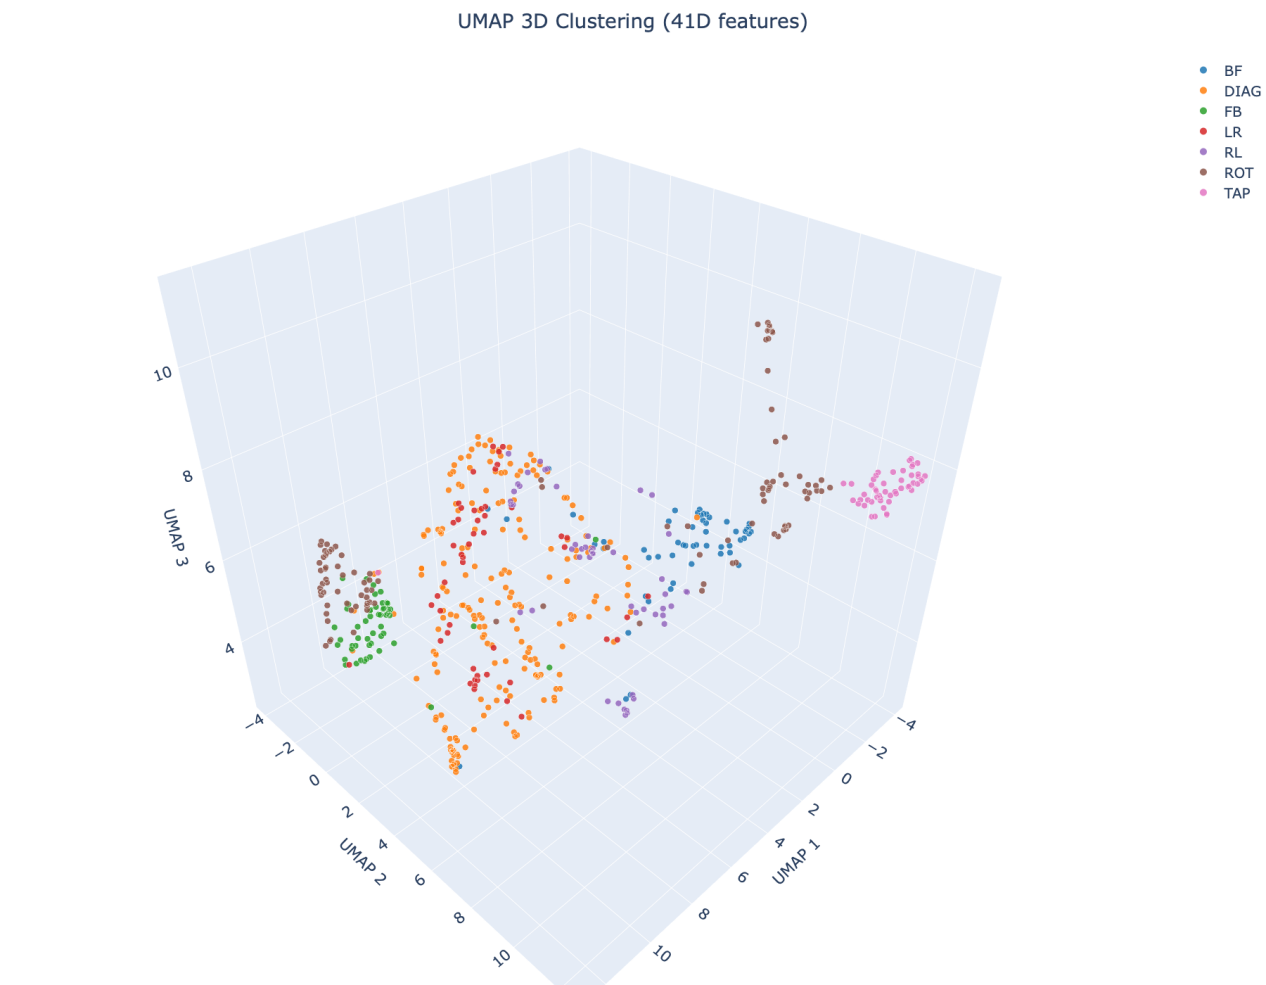
\includegraphics[width=0.85\textwidth]{doc_thesis/figs/04/umap_clustering.png}
    \caption{\ptheadingfont{SVM确定性信号聚类图}}
    \label{fig:umap_clustering}
\end{figure}

\begin{figure}[htbp]
    \centering
    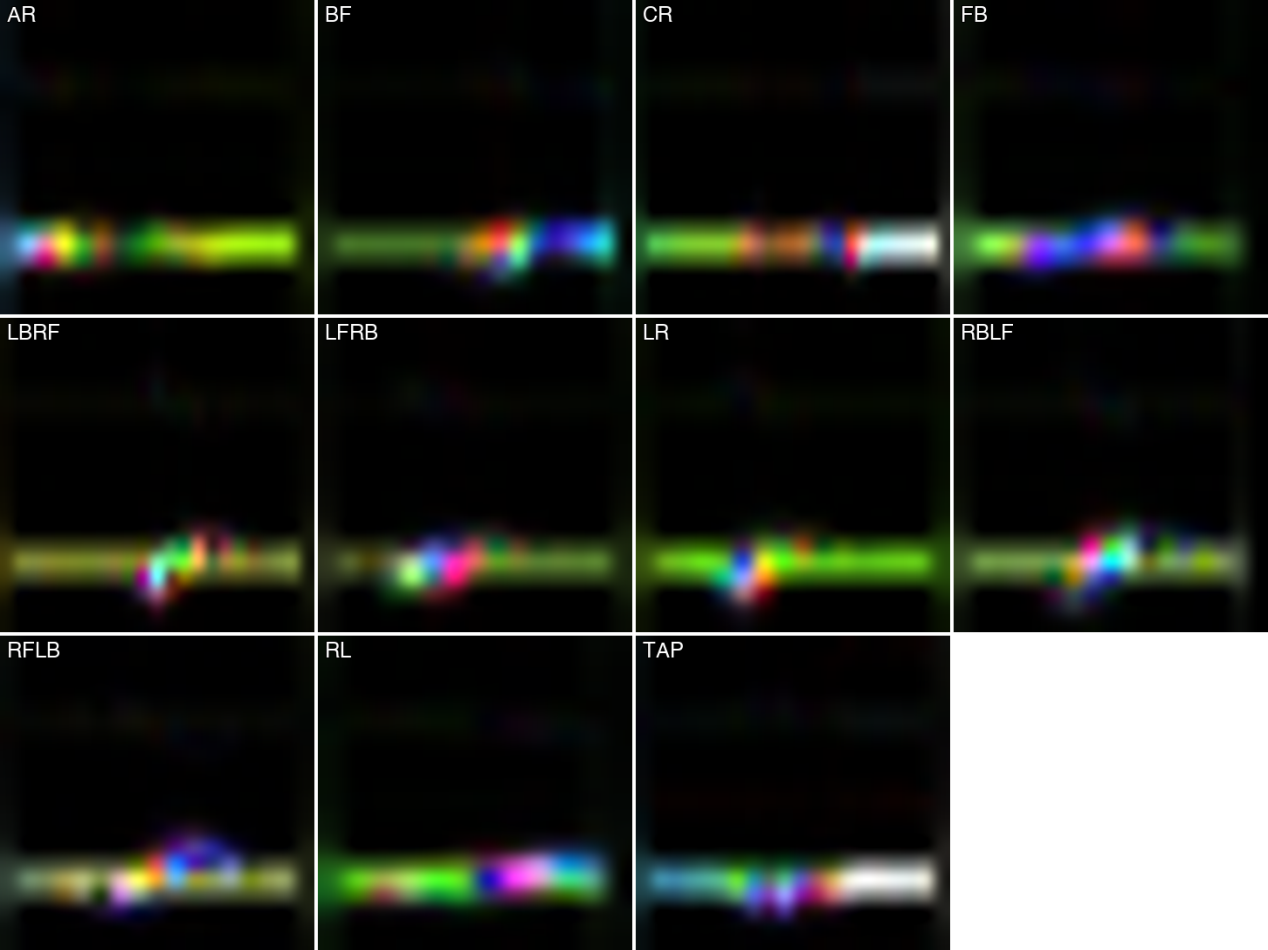
\includegraphics[width=0.85\textwidth]{doc_thesis/figs/04/spectrogram_grid.png}
    \caption{\ptheadingfont{手势信号混色频谱图}}
    \label{fig:spectrogram_grid}
\end{figure}

我们发现，对于非平动（比如转动），SVM系统的鲁棒性非常弱，尤其体现在确定性信号上，这与我们之前的理论分析相符合，也就是物理波长限制了对于微手势的识别，散射特性对角度极其敏感，相位特征稳定性下降。

\begin{figure}[htbp]
    \centering
    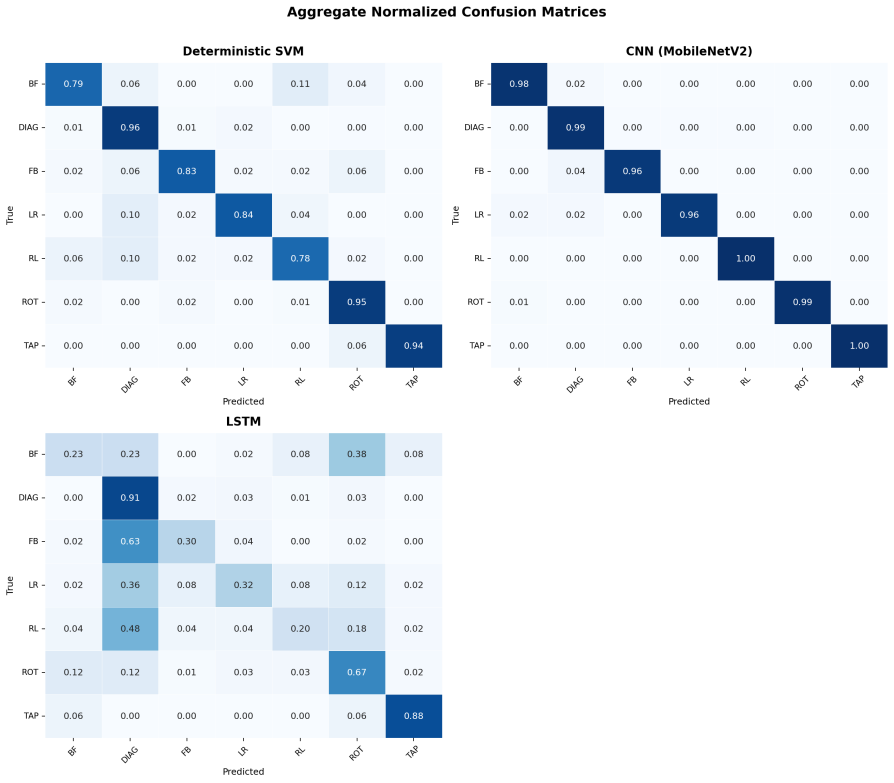
\includegraphics[width=0.7\textwidth]{doc_thesis/figs/04/confusion_matrices.png}
    \caption{\ptheadingfont{三种方法混淆矩阵对比图}}
    \label{fig:confusion_matrices}
\end{figure}

CNN 的混淆矩阵几乎接近单位阵（diagonal matrix，对角占优矩阵），混淆矩阵表现出显著的对角占优特性，大多数类别的识别准确率超过96\%。其中RL与TAP类别达到100\%的分类准确率，说明微多普勒频谱图中的局部纹理与时频结构能够被卷积核有效提取；而LSTM出现大量的非对角元素，说明时序特征在当前数据表示下未被有效学习；相比之下，尽管SVM未采用深度特征学习，其平均识别准确率仍达到90\%以上，说明基于确定性多普勒相位构建的低维特征向量已经具有较强的类别可分性。这表明本文提出的物理建模与特征提取方法能够有效压缩原始高维雷达信号中的判别信息。

频谱图中的速度变化轨迹、能量分布以及边缘结构具有明显的二维空间相关性，而卷积神经网络擅长提取局部纹理与空间模式，因此能够有效学习不同手势之间的判别特征；SVM模型的主要错误集中于具有相似运动轨迹或相近速度分布的动作类别之间。例如，LR与RL在频移方向上具有镜像对称关系，而BF与FB在时间反演后具有相似的频谱结构，因此容易发生类别混淆。

不同手势在雷达视角下会产生不同的径向速度变化过程，因此其对应的微多普勒谱图在频率扩展范围、能量聚集区域以及时间演化轨迹上呈现出具有物理意义的差异。这说明频谱图不仅是神经网络输入，更反映了手部运动学与电磁散射之间的映射关系。

综合来看，确定性信号分类+SVM的方法准确率90.1\%已满足实用需求，训练时间仅0.011s，可在CPU运行，端侧部署优势显著；准确率最高（98.4\%），但训练耗时最长（172.1s），且需要约1GB CUDA内存，适合云端部署；LSTM各项指标均最低，可能原因小样本场景（每类仅50--60样本）下黑盒模型易过拟合，并且时序模型对相位噪声敏感，缺乏物理先验引导。

\section{研究展望}

基于本研究的实验结果与局限性分析，后续研究方向聚焦在以下几个方面：

\begin{enumerate}
    \item 当前方法主要依赖相位极值时序特征，对旋转类手势（AR/CR）识别效果有限。未来可探索将幅度包络的时频特征与相位确定性特征进行早期/晚期融合，构建更完备的手势表征空间。

    \item 将米氏散射模型的几何约束（如相位演化凸性、极值点拓扑关系）作为正则项或注意力机制引入轻量神经网络，在保持可解释性的同时提升对复杂手势的泛化能力。

    \item 搭建小样本学习框架：针对新用户/新手势的快速适配需求，探索基于MAML或原型网络的小样本学习方案，实现"一次学习、快速迁移"。

    \item 5.8GHz波长（$\sim$5.2cm）与手掌尺寸相当，处于米氏散射敏感区。未来可探索双频（如24GHz+5.8GHz）或多频段可重构雷达，通过频率分集提升对不同尺度手势的适应性。

    \item 雷达信号虽不直接采集图像，但高分辨率回波仍可能泄露用户行为隐私。可研究在特征提取前端加入差分隐私或同态加密机制，实现"可用不可见"的感知范式。
\end{enumerate}

\section{结论}

毕业设计以三通道TDM-SIMO连续波多普勒雷达为硬件平台，围绕非接触式手势识别的理论建模、系统实现与算法设计三方面展开研究，完成了预期目标中的各项核心任务。

首先从米氏散射理论出发，分析了手掌作为较大尺寸目标在近场条件下的动态反射散射特性，推导了手掌运动速度、方向与各通道接收信号之间的确定性相位关系。基于该物理模型提取的功率峰值时间、DACM累积相位、通道间相位差等特征具有明确的物理含义，其对环境多径分量的天然抑制能力在实验中得到了验证——确定性信号方法无需额外的杂波抑制处理即可在多径环境下实现90.1\%的分类准确率。

随后搭建硬件链路端实现了稳定的高速采样，算法端构建了三种层次互补的识别方案：确定性信号特征结合SVM分类器实现了毫秒级的训练与推理（单次推理延迟0.33ms），CNN迁移学习方案达到了98.4\%的最高准确率，端到端推理延迟约6ms，均远低于200ms的实时交互阈值。系统成功实现了对前后、左右、对角线滑动、旋转及点击等7类典型手势的高精度分类。

针对连续交互场景中手势前后缺乏静止段的问题，通过利用连续信号流自动回溯静止区间恢复直流基线，并以功率峰值时间替代对边界敏感的相位最小值特征，在不牺牲交互自然性的前提下将确定性信号方法的准确率从约15\%提升至90.1\%。同时设计了灵活的类别合并机制，有效降低了运动轨迹相似手势间的混淆。

综上，毕业设计从电磁散射物理建模到系统实现再到算法优化，形成了完整的技术链路，验证了TDM-SIMO多普勒雷达作为下一代无感、私密人机交互接口的技术可行性，为非接触式手势识别从实验室走向实用化奠定了基础。
